\documentclass[tikz]{standalone}

\usetikzlibrary{positioning}

\begin{document}
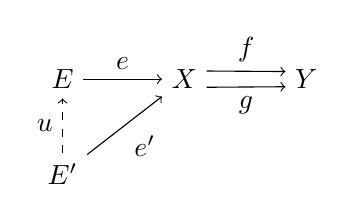
\begin{tikzpicture}
	\node (X) {$X$};
	\node [right=1.0cm of X] (Y) {$Y$};
	\node [left =1.0cm of X] (E) {$E$};
	\node [below=0.7cm of E] (E') {$E'$};
	\draw [->] (X.20) to node [above] {$f$} (Y.160);
	\draw [->] (X.340) to node [below] {$g$} (Y.200);
	\draw [->] (E) to node [above] {$e$} (X);
	\draw [->, dashed] (E') to node [left] {$u$} (E);
	\draw [->] (E') to node [below right] {$e'$} (X);
\end{tikzpicture}
\end{document}
